\newcommand*{\vttfamily}{%
\fontencoding{T1}\fontfamily{lmvtt}\selectfont
}

\newcommand*{\textsmallunderscore}{%
\begingroup
\fontencoding{T1}\fontfamily{lmtt}\selectfont
\textunderscore
\endgroup
}

\lstdefinestyle{codeStyleC}{
language=C++,
basicstyle=\ttfamily\small,
keywordstyle=\color{blue}\ttfamily,
stringstyle=\color{red}\ttfamily,
commentstyle=\color{green}\ttfamily,
breaklines=true,
columns=flexible,
gobble=4,
xleftmargin=\leftmargini,
frame=L,
numbers=left,
numberstyle=\tiny,
belowcaptionskip=0.5em,
belowskip=1em,
}

\definecolor{darkgreen}{rgb}{0,.5,0}
\lstdefinestyle{codeStyleCUDA}{
language=C++,
basicstyle=\ttfamily\small,
keywordstyle=\color{blue}\ttfamily,
keywordstyle=[2]\color{darkgreen},
keywordstyle=[3]\color{red},
stringstyle=\color{red}\ttfamily,
commentstyle=\color{green}\ttfamily,
breaklines=true,
columns=flexible,
gobble=4,
xleftmargin=\leftmargini,
frame=L,
numbers=left,
numberstyle=\tiny,
keywords=[2]{__global__,__host__,__device__,__synchThreads()},
keywords=[3]{atomicAdd},
belowcaptionskip=1em,
belowskip=1em,
}



\lstdefinestyle{codeStyleFORTRAN}{
language=FORTRAN,
basicstyle=\ttfamily\small,
keywordstyle=\color{blue}\ttfamily,
keywordstyle=[2]\color{darkgreen},
stringstyle=\color{red}\ttfamily,
commentstyle=\color{green}\ttfamily,
breaklines=true,
columns=flexible,
gobble=4,
xleftmargin=\leftmargini,
frame=L,
numbers=left,
numberstyle=\tiny,
keywords=[2]{__global__,__host__,__device__,__synchThreads()},
belowcaptionskip=2em,
belowskip=5em,
}





%chapter start here---------------------------





\chapter{Parallel GPU/CUDA Implementation of the lava flow model SCIARA-fv3}

\section{Introduction}
Parallel computing is a cost-effective method for efficient resolution of
problems and was used as tool for modeling real complex phenomena like a lava
flow, or snowflakes. Many techniques were developed in order to exploit the
power of parallelization differing from each other primarily for the underlying
parallel architecture they are designed for (see chapter
\ref{chap:parallelArchitectures}). In this work we adopted GPUs to accelerate
the SCIARA-fv3 lava flow  (see section \ref{sect:SCIARA_MODEL})cellular
automata model\footnote{A computational model proven to be very suitable for GPU
parallelization.} following the APOD parallelizing methodology (see section
\ref{sect:APOD}) and hence, different parallel versions of the model were
produced, incrementally adopting new features and strategies in order to
achieve better performances.

The versions produced have been:
\begin{description}
\item [\textbf{\textit{Na\"{i}ve implementation :}}] \hfill \\ A basic and simple porting
consisting in mapping each cell of the cellular space to a CUDA
thread. Most part of the scaffolding code was produced here because all the
algorithms and data structures, used in the serial code, that have prevented the parallelism
have been identified and handled (see section \ref{sect:topLevelStrategies} and \ref{sect:naiveImplementation}) .

\item [\textbf{\textit{Rectangular Bounding Box - RBB:}}] \hfill \\ A first
important optimization strategy was adopted here in order to mitigate the
problem of IDLE allocated threads (see section
\ref{sect:idleThreadsDevOccupancy}), that limits the occupancy of the device.
The computation is limited only within the boundaries of a rectangle that has
the property of containing all the active cells (see sections
\ref{sect:serialoptimization} and \ref{sect:RBBOptimization} ) \item
[\textbf{\textit{Shared memory utilization:}}] \hfill \\
A deep analysis on memory accesses was performed to select buffers and
variables more often accessed in kernel code in order to take advantage of the
shared memory (see sections \ref{shareMemory} and
\ref{sect:sharedMemoryOptimization}) \item [\textbf{\textit{Atomic function
implementation:}}] \hfill \\
A family of two versions exploiting CUDA \textit{atomic functions} was developed
as solution to the problem of race-conditions while distributing flows among
cells (see algorithm \ref{alg:distribution})
\begin{enumerate}
  \item \textbf{\textit{RBB-atomic}} : A porting of the RBB version
  introduced before without utilizing the flow's substates (see section \ref{sect:raceCondAvoiding}) for lava flow
  distribution.
  \item \textbf{\textit{List active cells and atomic functions}} : IDLE cells
  and related IDLE threads have been found to be the most prominent limiting
  factor in exploiting GPU power. This version implements a mechanism that tries
  to avoid almost completely this issue, showing very good improvements in
  performances (see section \ref{sect:linearCellAtomic}).
\end{enumerate}
\end{description}


%\subsection{Previous works}
%\label{previousWork}




\section{The Assess, Parallelize, Optimize, Deploy (APOD) design
cycle}\label{sect:APOD}
The Assess, Parallelize, Optimize, Deploy (APOD) is a
cyclical process strategy in parallelizing code. It allows initial speedups to be achieved, with
only minimal initial investment of time (is common that a na\"{i}ve porting of the
application appears to be very easy). The application can be tested, and deployed
at which point the cycle can begin again by identifying further optimization
opportunities, seeing additional speedups, and then deploying the even faster
versions of the application(see figure \ref{fig:APOD}).


\begin{figure}
\begin{center}
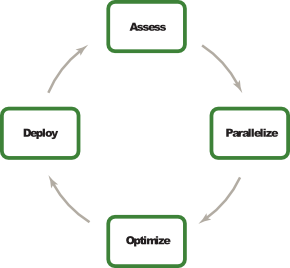
\includegraphics[scale=0.85]{./images/apod-cycle}
\caption[APOD]{APOD design cycle process}
\label{fig:APOD}
\end{center}
\end{figure}

\subsection{Assess}
In this phase, for an existing project the first step is to locate parts of the
code that are responsible for the bulk of execution time, trying to evaluate
bottlenecks and less adapt GPU parallelization parts (see section
\ref{analysysserialCode}).
This way of thinking is a direct consequences of the Amdahl's and Gustafson's
laws (see section \ref{sect:profiling}), and moreover thanks to them the
developer can determine an \textbf{upper bound} of performance improvement from acceleration
of the identified hotspots.

\subsection{Parallelize}
Once hotspots have been identified the developer has to start to parallelize
the code. Depending on the application this goal can be achieved just calling
accelerated libraries (in GPUGPU CUDA environment e.g. cuBLAS or Thrust) or
adding preprocessor directives (e.g. OpenACC or OpenMP). On the other hand,
sometimes in order to fully expose inherent program's parallelism the parallel
porting require some amount of refactoring of the existing serial code.

\subsection{Optimize}
After each round of parallelization the developer can think and move to further
optimize the application. Optimizations can be applied incrementally, and can be
tested in term of speedup achieved and validated.
Optimization can be applied at different level: from the overlapping of memory
transfers with computation to the best block-grid dimensions for a
given kernel in order to augment the occupancy. Profiling and debug tools are
invaluable for this stage of the process as they can suggest the next-best
course of action and provide vital information about the performances.

\subsection{Deploy}
In this phase the developer can compare the outcome with the original
expectations (determined at the \textit{assess} phase). Partial parallelized
program can be carried out for production (this is more important within an
industrial context, because clients can take profit from their investments as
early as possible).

\section{Analysis of the serial code}\label{analysysserialCode}
Undoubtedly, a solid theoretical understanding of the mathematical model and of
the program that actually implements that model (if already exists) are the very
first crucial steps in the process of porting any parallel software.
If the parallelization work starts from an existing code, an analysis phase of
the code itself is fundamental, the reason why this work started from this point.
Cellular automata are well suitable for parallelization, even on GPUs, so the
purpose of this phase is not to determine whether or not the problem is one that
can actually be parallelized but, to identify the program's
\textbf{\textit{hotspots}}, portions of code where most of the work take place
\footnote{Usually scientific and technical programs accomplish most part of the
work, in terms of execution time, is concentrated in few procedures, and
constitute a tiny amount of the whole source code.} and hence concentrates on
parallelizing these hotspots, ``ignoring'' those section of the program that
are not compute intensive in terms of FLOPS. Another important phase is to
identify bottlenecks, areas that could cause parallelizable work to halt or
slowdown (I/O operation are usually something that prevent a full exploiting of
the parallelism, or data dependences), and to possibly restructure those
sections using new approaches, or different algorithms to reduce or eliminate
those bottlenecks.

For example, the problem of calculating the Fibonacci series\footnote{A
particular case of the Fibonacci polynomials F_n(x)=xF_{n-1}(x)+F_{n-2}(x)\)
s.t. \(x=1\) The famous sequence starts with the number 0 and 1 and each
subsequent number is the sum of the previous two. } defined as:
\[ F(n)= F(n-1)+F(n-2), \:\: s.t. \: F(0)=0\;,F(1)=1 \] \[ F(0)\ldots F(17):0,
1, 1, 2, 3, 5, 8, 13, 21, 34, 55, 89, 144, 233, 377, 610, 987, ...
\] is a good example of how an algorithm can deny the parallelization of a
problem. We can see that this approach exposes a too strong data dependence
condition among the values of the series that disallow any possible parallel
implementation because each \(F(n)\) cannot be calculated independently, and
indeed depends of the previous two calculated values.
For example : \hfill \\
\( F(4) = F(4-1)+F(4-2) = (F(4-2)+F(4-3))+(F(4-3)+F(4-4))=
F(4-3)+F(4-4)+F(1)+F(1)+F(0)=F(1)+F(0)+F(1)+F(1)+F(0)=1+0+1+1+0=3 \) to
calculate the \(4\)th element of the series this algorithm needs the 3th and the
2th value. They recurrently need the 2th the 1th, the 0th and so on. It is worth to note that it could be
convenient in this case to change the computation algorithm and using instead of
a recurrent function, a closed formula like the Binet's Fibonacci numbers
formula :
\[ F(n)=\frac{{(1+\sqrt{5})}^n-{(1-\sqrt{5})}^n}{2^n\sqrt{5}} \] or one that use
golden ration \(\phi\) \cite{Wells1986}:
\[ F(n)=
\begin{bmatrix}

\frac{\phi^n}{\sqrt{5}}

\end{bmatrix}
\]
that enables a fully parallelized implementation to take place, enabling two or
more processor to calculate in parallel chunks of the series.

\subsection{Serial code overview}
In this section we'll try to get more into the details of the serial
implementation, in order to better explain the choices taken in parallelizing
the code.


\subsubsection{Memory Organization and data structures}
Working on bi-dimensional cellular automata is not surprising if the
underlying representation of the set \(Q\) of substates is
bi-dimensional as well (see listing \ref{code:memoryPattern2D}) and hence
implemented as:

\lstset{label={code:memoryPattern2D},caption={Substates allocation in serial
code}, style=codeStyleC }
\begin{lstlisting}
	// Substates
	double **Sz;	//Altitude
	double **Sh;	//Lava thickness
	double **nSh;
	double **ST;	//Lava temperature
	double **nST;
	double **SEk;	//Kinetic energy
	double **nSEk;
	\end{lstlisting}
a series of double canonical dynamical C/C++ matrixes for each
substate (we'll see in section \ref{1Dto2Dmemory}
that this memory setting is problematic in CUDA), one for reading cell neighbor
(\textit{updatedCA}) substates and a second for writing the new substate values
(\textit{currentCA}).

Parameters are organized as a series of scalar variables:

\lstset{label={code:memoryPattern2D},caption={}, style=codeStyleC }
\begin{lstlisting}
	double Prho;		//density
	double Pepsilon;	//emissivity
	double Psigma;		//Stephen-Boltzmann constant
	double Pcv;			//Specific heat
\end{lstlisting}

while an abstraction of the vent is given by the class \texttt{TVent} that
encapsulates the class \texttt{TEmissionRate} which store the values, variables
and methods to represent a particular vent emission rate.
The main function of the vent abstraction class is to give back an amount of
produced lava after a certain amount of simulated event's time. The emission of
lava from the vent was discretized into time slot of \(t_e\) and it means that when the simulation time
\(t_s\) is such that \(i t_e \leq t_s < (i+1)  t_e \) the emitted lava thickness
value at the slot number \(i\) is returned.
\lstset{label={code:memoryPattern2D},caption={}, style=codeStyleC }
\begin{lstlisting}
	double thickness(double sim_elapsed_time, double Pt,unsigned int emission_time,
	double Pac) { 
	unsigned int i = (unsigned int)(sim_elapsed_time/emission_time); 
	if (i >= _emission_rate.size())
		return 0;
	else
		return _emission_rate[i]/Pac*Pt;
	}
\end{lstlisting}


\subsubsection{Transition function and elementary processes}
The transition function \(\tau\) and all the elementary processes \(
\tau_1,\tau_2 \ldots \) have  correspondent functions in the code.
\lstset{label={code:memoryPattern2D},caption={}, style=codeStyleC }
\begin{lstlisting}
	void GlobalTransitionFunction();
	void SwitchToHeat();
	void empiricalFlows();
	void getInitialVelocities(const int& x, const int& y, double* v);
	double outflowsProp(int x, int y, double *f, double *v, double *p, bool T_or_F);
\end{lstlisting}

The transition function consist of ordered calls to the \(\tau_1,\tau_2 \ldots
\) procedures. One of them, \texttt{empiricalFlows()}, is more interesting than
the others because it involves the determination of the temporal step, the
calculation of the superficial flow and their distribution among the cells in
the neighborhood of a central cell.
As stated in section \ref{sect:modeltimeEvaluation} the temporal
computational step is the minimum between all the temporary computational time
step calculated by each cell and the distribution is outlined in the algorithm
\ref{alg:distribution} (for the sake of brevity taking in account only one
substate, the lava thickness, but the same strategy is applied also to the
others):

\begin{algorithm}
\begin{algorithmic}

\FORALL {$c \leftarrow cell$}
\FORALL {$n \leftarrow  neighborhood(c)$}

\STATE $nSh(c) \leftarrow nSh(c)-flow(c,n)$
\STATE $nSh(n) \leftarrow nSh(n)+flow(c,n)$

\ENDFOR
\ENDFOR
	\caption{Distribute lava flow among the neighborhood's cells}
	\label{alg:distribution}
\end{algorithmic}
\hfill\\

where \texttt{flow(c,n)} is the computed superficial flow of lava from the cell
$c$ to the cell $n$ and \texttt{nSh(c)} is the update matrix of the substate thickness.
The lava flow from the central cell \(c\)
to a cell $n$ of the neighborhood is subtracted (reason of the minus sign),
and added to cell $n$ itself.
\end{algorithm}
Two important information arise from the analysis of this function:
\begin{itemize}
  \item At each step a minimum value has to be found among all the cell of
  the cellular space; in a parallel context this should be carried out by means
  of some reduction algorithm.
  \item This distribution approach is not suitable for a direct porting due to
  the obvious race condition problems.
\end{itemize}
We will take in account these and other problems in section
\ref{sect:raceCondAvoiding}.

\subsubsection{Serial Optimizations}\label{sect:serialoptimization}
This way of updating the cellular space, although it does not fit perfectly with
the theoretical cellular automata model, may be considered as an optimization
because otherwise a set of nine flow substates should be stored and managed to
keep track of the substates quantities interchanged at each step.
Moreover the transition function is applied only on cells where the thickness
substate value \(sh_{cell} > 0 \). The cellular space could be formed by a very
large number of cells (for example we applied the model to a discretization of a
flank of Mount Etna corresponding to a \(517 \times 378 = 195426\) cells
cellular space), but in the context of ``evolutive'' phenomena such as volcano
eruptions and consequent lava flow modelling, that evolve starting from only a
limited active part of the space and growing as the time passes by, cells that
are far from lava are considered to be \textit{idle} because they cannot be
neither sources nor receivers of any lava quantity, consequently skipping their
computation would not affect the final result. Hence minimizing the number of
times in which transition function is applied on idle cells could be crucial for
performances and in a serial programming context this can be accomplished easily
without any overhead.
The listing \ref{code:skypIdleCell} shows how a serial implementation of the
cellular automata loops over the cellular space and it selectively applies the
transition function whether the \texttt{if} predicate \(sh_{cell} > 0 \) is
true.
The most computationally intesive part of the transition function is so avoided
for such cells.
\lstset{label={code:skypIdleCell},caption={Selective applying of the transition
function on active cells.}, language=C++, basicstyle=\footnotesize\ttfamily,
keywordstyle=\color{blue}\ttfamily, keywordstyle=[2]\color{darkgreen},
stringstyle=\color{red}\ttfamily, commentstyle=\itshape\color{green},
breaklines=true, frame=L, columns=flexible, gobble=4, xleftmargin=\parindent,
belowcaptionskip=1em, belowskip=1em, }
\begin{lstlisting}
	for (int x = 0; x < COLS ; x++)
		for (int y = 0; y < ROWS ; y++)
		if (Sh[x][y] > 0 ) {
			...
			/*HEAVY WORK*/
			...
\end{lstlisting}


Hence from here it's clear that the minimization of the idle cells computation
is an important optimization and we'll see in sections \ref{sect:RBBOptimization} and
\ref{sect:linearCellAtomic} that this idea is still valid in a parallel context.

\subsection{Profiling - Gprof}\label{sect:profiling}
Bottlenecks can be identified by performing the profiling analysis of the code.
Profiling consist of a numbers of metrics that describe the complexity of an
application in term of space and time. Profiling is achieved using tools called
\textit{code profilers}.
The output of a profiler usually consist of a :
\begin{description}
\item[Statistical summary:]\hfill \\
The profiler annotates statistics and metrics against the source
code statements when a certain event occurs (e.g. a method call or an
\texttt{else} part of a \texttt{if} branching). It can record for example the
entire trace of the called methods in a so called \textit{call graph} (see figure \ref{stackCall}). A call
graph is a direct graph describing relations between subroutines. It could be:
\begin{itemize}
  \item \textbf{dynamic}
  Is dynamic when the graph is a record of an execution of the program.
  \item \textbf{static}
  Static call graph are built ``offline'' and it intends to represent
  \textbf{every} possible run of the program. Building an exact static call
  graph is an undecidable problem so usually they are approximations. An
  example of tools that perform static call graph analysis are
  \textit{cflow}\footnote{\url{https://lists.gnu.org/archive/html/info-gnu/2011-10/msg00010.html}}
  and
  \textit{egypt}\footnote{\url{http://www.gson.org/egypt/}}
\end{itemize}
\end{description}

For this work the profiling tool Gprof was used. It is a Unix tool that allows
to compute a large number of statistics and a dynamical call graph. There was no
need for any static graph call analysis because the purpose of using a profiling tool was not to
understand the behavior of the program but to find the possible bottlenecks and
hotspots. It works injecting instrumentation code automatically into the code (
compiling\footnote{Gprof can be used only with compatible compilers like G++}
with the option \textit{-pg}) like for example a call to a monitor function
\textit{mcount}\footnote{This function may not be thread safe in some
implementation, so can produce incorrect results.} before each function call.
At the end of the execution a file with extension \textit{.gmon}
(program\_name.gmmon) is saved.
The information is collected simply sampling the execution of the program
probing the target program's \textit{program counter} at regular intervals using
operating system interrupts (programmed via \texttt{profil()} or
\texttt{setitimer()} syscalls).
The overhead related to the profiling with Gprof can vary from 30\% to 250\%
\cite{Froyd2005}.




\subsection{SCIARA-fv3 profiling}
In figure \ref{stackCall} the call graph\footnote{The stack call image was
obtained using the script GProf2Dot that convert profiling output from Gprof to
a dot graph. \url{https://code.google.com/p/jrfonseca/wiki/Gprof2Dot}} coupled
with other metrics is shown as the number of times that a function is called
and the percentage of the total time that a use (we omitted, without losing any critic
informations, functions which the execution time was too short or not directly
related to the computation, e.g. initialization of threads or setting up of
linked list because of readability).
The figure is related to an execution of \(2000\) computational steps of the
model itself.
We can easily see that the \textbf{97\%} (i.e. it may allow a almost fully
parallel implementation) of the computation takes place into function
\texttt{GlobalTransitionFunction()} that is called in total, not surprisingly
2000 times. The top level hotspot is so identified and we can start making some
prediction about the speedup's upper bound according to the Amdahl's law.
Using \(p=512\) cores of a fermi GTX 580 GPU we can expect that the speedup \[
S(512)=\frac{1}{B+\frac{1}{512}(1-B)}\approx31.35, \quad B=1-0.97; \] where B is
the serial portion of the whole program. We cannot expect speedups better than
\(31\times\) even using 512 cores in parallel and without any additional
overhead (at least on 2000 computational steps).
Obviously as the computational steps increase the percentage of the total time
taken by the hotspots \texttt{GlobalTransitionFunction()} becomes closer and
closer to \(100\%\), giving at limit a theoretical speedup limit \(S(p)=p\).
Hence, all the efforts in parallelizing the application have been spent on the
acceleration of this part. Each called procedure in
\texttt{GlobalTransitionFunction()} procedure corresponds to an elementary
process\footnote{We can easily see from the same figure that the most
computationally expensive, among them, is the calculation of the outflows
called 9 times for each cell and computational step.} of the MCA.
\begin{figure}[p] \vspace*{-2cm}
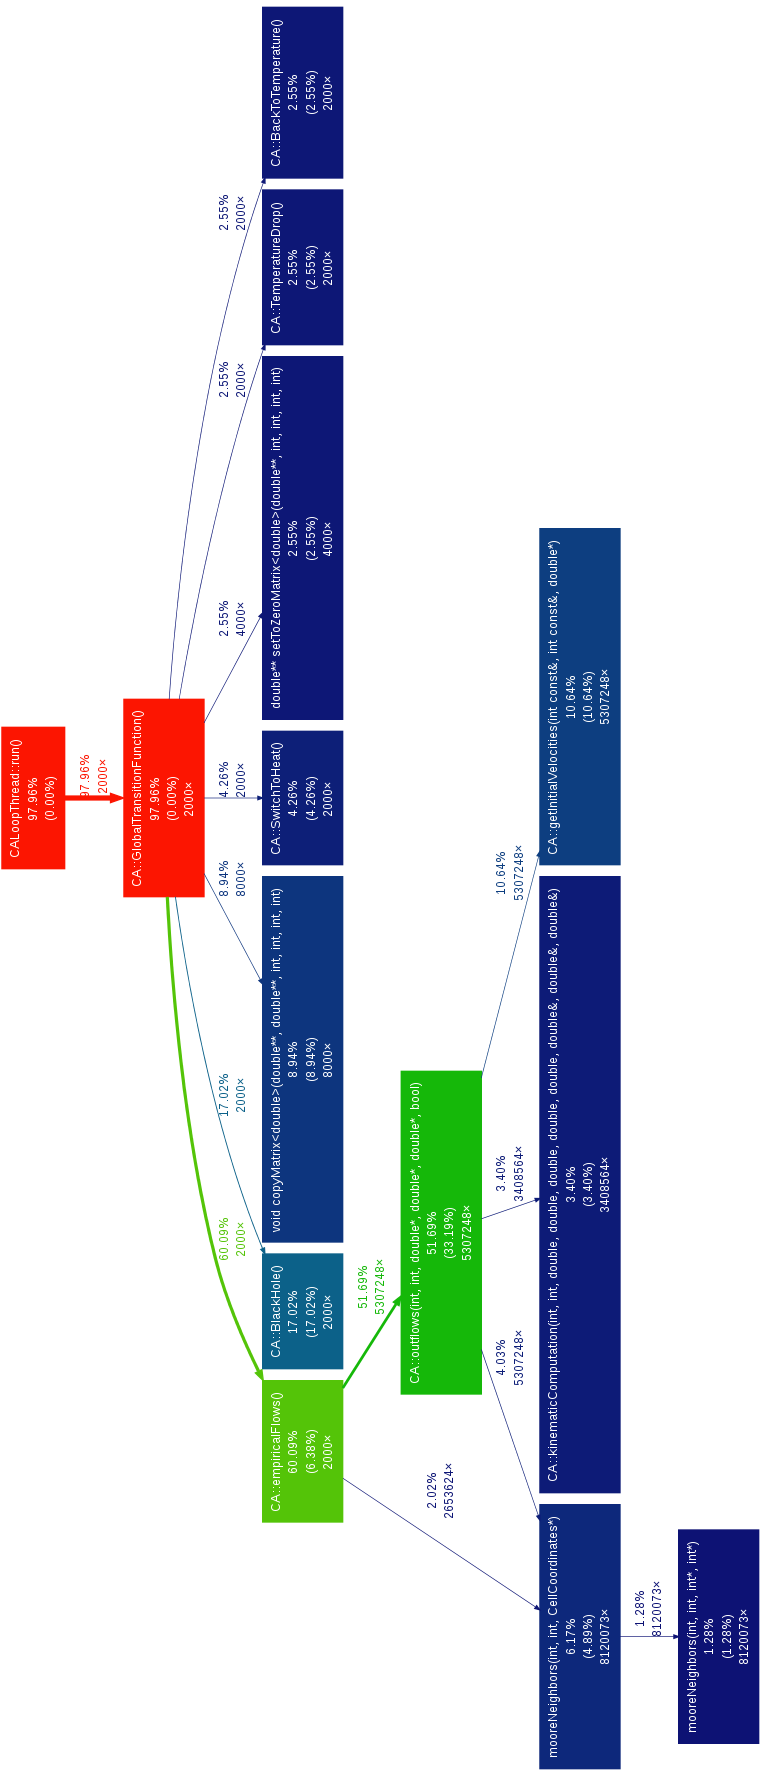
\includegraphics[width=0.67\linewidth]{./images/profiling}
\caption{Call graph for the serial version of the SCIARA-fv3 model}
\label{stackCall}
\end{figure}
Another important information  obtainable from the figure \ref{stackCall} is
that the bulk of computation  is not enclosed in one single very computationally
intensive procedure call (like, for example, could be a single call to a
matrices multiplication, or a differential equation solver procedure), but it
resides in the large number of calls to sub-procedures, (\(\approx5\times10^6\)
calls for the sub-procedures like \texttt{outFlows(\ldots)} in this specific run
of the model).




\section{Top level and strategies overview}

\label{sect:topLevelStrategies}
At high level the workflow of the parallel version consists of (the classic
host-managed accelerated program structure):
\begin{enumerate}
  \item Data structures initialization on CPU (see section \ref{1Dto2Dmemory})
  \item Memory copies \(CPU \rightarrow GPU\)
  \item Global transition function execution on GPU
  \item Results memory copies \(CPU \leftarrow GPU\)
\end{enumerate}

The parallelization strategy design purpose was to avoid as much as possible the
highly undesirable \(CPU \leftrightarrow GPU \) copy operations by means of a
complete execution of all the elementary processes functions on the device and
performing only a \(updatedCA \leftarrow currentCA \) device-to-device copy
operation to re-initialize the \textit{updatedCA} swapping the latter with the
\textit{currentCA} buffers (see section \ref{sect:serialoptimization}).

The elementary processes are the constituent of the global
transition function of the cellular automata and the order in which they are
executed is crucial for the correctness of the final result. They need to be
applied sequentially and hence \(\tau_{i+1}\) can be applied only and only if
\(\tau_{i}\) was already executed. From an implementation point of view this
means that all cells have to first compute the current elementary process before
performing the subsequent one. Hence we decided to map each elementary process
to different CUDA kernels that allow a global synchronization (at grid level),
not interleaving (as soon as they are executed on the same CUDA stream), de
facto, any elementary process function. An example is shown in listings
\ref{code:kernelCalls}.

\lstset{label={code:kernelCalls},caption={Elementary processes kernel
function calls.}, language=C++, basicstyle=\footnotesize\ttfamily,
keywordstyle=\color{blue}\ttfamily,
keywordstyle=[2]\color{darkgreen},
stringstyle=\color{red}\ttfamily,
commentstyle=\itshape\color{green},
breaklines=true,
frame=L,
columns=flexible,
gobble=4,
xleftmargin=\parindent,
belowcaptionskip=1em,
belowskip=1em, }
\begin{lstlisting}
	//crater kernel
	handleVents<<<1,sciaraGPU->params[EN_numVents]>>>(...);
	
	//elementary process #1
	switchToHeat<<<dimGrid,blockSize>>>(...);
	
	//elementary process #2
	empiricalFlow_fill_TIMES<<<dimGrid,blockSize>>>(...);
\end{lstlisting}

In order to exploit the fine-grain parallelism of the CUDA architecture one of
the first issues to decide is the amount of work that a single thread has to be
loaded with, in term of numbers of cells that it has to take into account. For
example one might think to use one thread for a single row or column or in
general for a subset of the cellular space as in a typical data-parallel
application. However while working with CUDA a very high number (thousand or
even millions) of threads should be created in order to exploit the massive
parallel architecture of the GPU\cite{NvidiaprogGuide}. The most common and
widely adopted strategy while working with arrays in CUDA is to map one thread
to one cell and similar approaches are used for example in \cite{dambrosio2012}.
The thread grid and blocks dimension have to be setted to the best value
according to CUDA best practices\cite{CUDACBESTPRACTICE} manual and choosed
utilizing the CUDA provided occupancy calculator spreadsheet (see
\ref{sect:cudaPerfGuideline} at page \pageref{sect:cudaPerfGuideline}). Those
values change from kernel to kernel, and depend on the device actually utilized
and on a number of other factors like the register pressure or the shared memory
utilization. In addition to this analysis, a series of experimentations were
performed in order to find the best set of values to achieve best performances. 
The transition function code may be very thread divergent because of the
complexity of the physical simulation. Another example could be
the if statement, that limits the execution only to the \textit{active} cells,
as talked in section \ref{sect:serialoptimization}.
At step \(t\) the lava is not homogeneously distributed among all the cells, and
it means that it is possible, for two different threads (i.e. cells) in the same
warp, to execute two divergent code paths. In sections
\ref{sect:atomicImplementation}, \ref{sect:RBBOptimization} and
\ref{sect:linearCellAtomic} we discuss some possible solutions in order to
mitigate this issue.
In listing \ref{code:threadDivergentCode} we show an example of a very thread
divergent code within SCIARA-fv3: a multiple \texttt{if-else} inside a loop. Each
thread within a warp can execute a different path at each iteration of the loop at line 1, preventing CUDA to fully
parallelize this section, and executing in serial the thread's subsets of the
warp in which all the threads share the same divergent path. Each subset is then
executed in parallel. In the worst case, when all the threads within a warp
execute a different path, the executions is completely serialized\footnote{CUDA
is SIMT because allow divergent execution path, but, it does not come for free.
A certain amount of serialization is the price to relax the strict SIMD
programming rules, and hence, a good CUDA programmer should avoid as much as
possible those divergent execution paths.}\cite{NvidiaprogGuide}.





\lstset{label={code:threadDivergentCode},caption={Thread divergence code, into
the calculate outflows elementary process function.}, language=C++,
basicstyle=\footnotesize\ttfamily, keywordstyle=\color{blue}\ttfamily, keywordstyle=[2]\color{darkgreen}, stringstyle=\color{red}\ttfamily,
commentstyle=\itshape\color{green},
breaklines=false,
frame=L,
columns=flexible,
gobble=4,
xleftmargin=\parindent,
belowcaptionskip=1em,
keywords=[2]{__constant__,__global__,__host__,__device__,__synchThreads()},
belowskip=1em, }
\begin{lstlisting}
    for (int i = 1; i < MOORE_NEIGHBORS; i++) {
	i < VON_NEUMANN_NEIGHBORS ? zc[i] = z[i] : zc[i] = z[0]-(z[0]-z[i])/rad2;

	// ha and he evaluation
	if (z[0] + hkr + hk[i] + h[0] <= zc[i] + h[i]) {
		he[i] = 0;
		ha[i] = h[0];
	} else if (z[0] + hkr + hk[i] >= zc[i] + h[i]) {
		he[i] = h[0];
		ha[i] = 0;
	} else if (z[0] + hkr + hk[i] + h[0] > zc[i] + h[i]) {
		he[i] = (z[0] + hkr + hk[i] + h[0])-(zc[i] + h[i]);
		ha[i] = h[0] - he[i];
	}
	i == 0 ? w[i] = 0 : w[i] = Pc;
	theta[i] = atan(((zc[0]+ha[i]+he[i] / 2.0) - (zc[i]+h[i])) / w[i]);
	w[i] = w[i] / cos(theta[i]);
	}

\end{lstlisting}

Regarding the mapping between the data structures and the CUDA memories we
followed the CUDA best practice manual\cite{CUDACBESTPRACTICE} advices.
Substates are arrays whose dimensions are only suitable for global memory
memorization whilst for parameters we decided to utilize constant memory (see
section \ref{sect:constantmemory} at page \pageref{sect:constantmemory}) due to
their intrinsically constant nature and their access rate in the code.
Moreover, all the constant variables of the automata have been stored in this
memory like for instance \(x\) and \(y\) dimension's sizes of the cellular space
which, although not strictly parameters, are constant while
the execution of the model, from the beginning to the end of the simulation. In listings
\ref{code:constantDeclaration} the declaration of the array stored in constant
memory is shown.
Note that it is an automatic array, and its dimension has to be known at compile
time and so an analysis phase was needed to select all the candidate variable to
be stored in that buffer.

\lstset{label={code:constantDeclaration},caption={Thread divergence code, into
the calculate outflows elementary process function.}, language=C++,
basicstyle=\footnotesize\ttfamily, keywordstyle=\color{blue}\ttfamily, keywordstyle=[2]\color{darkgreen}, stringstyle=\color{red}\ttfamily,
commentstyle=\itshape\color{green},
breaklines=false,
frame=L,
columns=flexible,
gobble=4,
xleftmargin=\parindent,
belowcaptionskip=1em,
keywords=[2]{__constant__,__global__,__host__,__device__,__synchThreads()},
belowskip=1em, }
\begin{lstlisting}
	#define NUM_PARAMS 21
	enum { EN_Pc1, EN_Pac1, EN_PTsol1, ... ,EN_LX1,EN_LY1};	
	__constant__ float d_params[NUM_PARAMS];

\end{lstlisting}


The main program and all the kernels are organized in C style manner in the
sense that CUDA does not allow C++ features such as classes utilization in its
code.
Thus, two c-99 structs have been created and combined to recreate the serial SCIARA-fv3 object
structure. They store a double copy of all the data, a CPU and GPU
version\footnote{Note that those double copies are different from the pair of
buffers that are needed for updating the next CA configuration at each step.
Here we are referring to a mirror copy of each variable we find in GPU device memory,
because at the beginning, at the end and sometimes in the middle of the
execution we need to perform some buffers copies that require a CPU version of
the buffers.}.
The original data structures are first copied into the new CPU data structures
in order to be copied and mapped into the GPU buffers.

\begin{enumerate}
  \item \texttt{SCIARA\_GPU}  : Main struct of the model, in which all the
  data structures are declared, created and destroyed. It is provided also with
  a method that allows the initialization of all the buffers from the CPU
  version of the model (that actually do the reading of all the initial
  configurations and parameters). It also contains an instance of the structure
  \texttt{SCALAR\_GPU}, that manages all the scalar values.
  \item \texttt{SCALAR\_GPU}: All the scalar values and methods that are related
  to them (like truncation or mathematical operations) are stored in this
  structure.  It is enclosed into the main structure of the program and managed by it.
\end{enumerate}

As stated in section \ref{sect:APOD} the assess phase of the development
consists also in locating possible parts of the code that are not very suitable for a
parallel implementation, either in terms of possible race-conditions or strategy
and algorithms, adopted in the serial version, that could limit the total amount
of parallelism that can be achieved. The most evident parallel implementation
limitation is related to the bi-dimensional data structures used in the serial
version. In the following section \ref{1Dto2Dmemory} we discuss more in detail
this issue and its solutions.

\subsection{Migration from 2D matrices to linear arrays}
\label{1Dto2Dmemory}
The first problem that was faced regarded the data organization in memory.
2D matrices are not allocable in the CUDA framework, which gives only the
possibility to allocate linear arrays within the global memory
\ref{memoryModel}. We first produced a serial version of the model that uses
only 1D arrays using an explicit row-major representation\footnote{Row-major is the internal
memory representation adopted in C/C++ languages to store automatic matrix
that are stored in a linear e continuous space in memory. Dynamic matrices are
usually managed allocating vector of pointers each representing a row. This
approach only store the data within a row in contiguous space, but spread the
rows into the heap space}; it involves the transformation of the cell
coordinate from 2D to a scalar number.
Given a 2D matrix of dimension \(D_y,D_x\) where \(D_y\) is the number of
rows and \(D_x\) is the number of columns and a cell of 2D coordinates
\(C_{2D}=(y,x)\) the scalar 1D coordinate is obtained using \(c_{1D}=yD_x+x\).
Cells are stored in a linear array such that rows are memorized one after the
other.
For example see figure \ref{fig:rowMajor}. 
\begin{figure}
\begin{center}
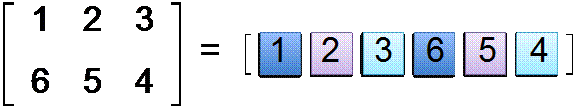
\includegraphics[scale=0.45]{./images/rowmajor}
\caption{Row-major matrix translation}
\label{fig:rowMajor}
\end{center}
\end{figure}
\FloatBarrier
Note that the same concept of ordering cells in 1D buffers is applicable also to
n-dimensional arrays \(n > 2\).
\subsubsection{Row-Major n-dimensional arrays representation}
Generalizing : If \(A=D_1 \times D_2 \times  \ldots \times D_n\) is a
n-dimensional array and given an element of A specified by a n-tuple \(a=(d_1,d_2,\ldots,d_n)\)
of (indexing start from zero) where \(d_k \in [0, D_k-1]\), the
memory offset in a 1D representation of A is:
\[
offset=\sum_{k=1}^{n}\left ( {  \prod_{l=k+1}^{n}D_l}\right )  d_k
\]

Intuitively a \(n-\)dimensional topology can be thought as series of \(D_n\)
topologies of \(n-1\) dimensions each like a 3 dimensional array as a
collection of ordered 2D matrices.
An offset \(o\) is a linear index of a cell in 1D coordinates that correspond
with its position in one of all the possible enumerations of the structure's
cells. For example the \(6\) in figure \ref{fig:rowMajor} is the 4th element in
row-major enumeration that sorts the indices by their dimensions from first to
last. In another enumeration, as column-major, where the sorting proceeds from
last to first, this element would have the 1D index 2.

Ordering from first to last means that, if a cell has coordinates \(d_n=k, \;
D_k\) structures of dimensions \(n-1\) have been already indexed and enumerated.
For example in a 3-dimension array of size \((D_1,D_2,D_3)= (10,8,7)\), a cell
of coordinate \((d_1,d_2,d_2)=(3,4,5)\)  is enumerated after \(d_1=3\) whole 2D
matrices of dimension \((D_2,D_3)=(8,7)\). The same concept recursively can be
used now to count the 2D element of coordinates \((d_2,d_3)\) in the 2-dimension
structure which its belongs. This cell is enumerated after \(d_2=4\) rows each
of dimension \(D_3\). The last dimension can be treated as an 1D array itself,
and is enough to add the value of that coordinate to the total count to obtain
the final offset. Hence the expansion for the 3D example is:
\[ o=d_1 \cdot (D_2 \cdot D_3) + d_2 \cdot (D_3) + d_3 = 3 \cdot (8 \cdot 7) + 4
\cdot 7 + 5= 201 \] meaning that the cell is located 201 cells after\footnote{To
be precise \(201 \cdot sizeof(data type)\) bytes after the pointer to the buffer.}
the buffer begin.
\begin{figure}
\begin{center}
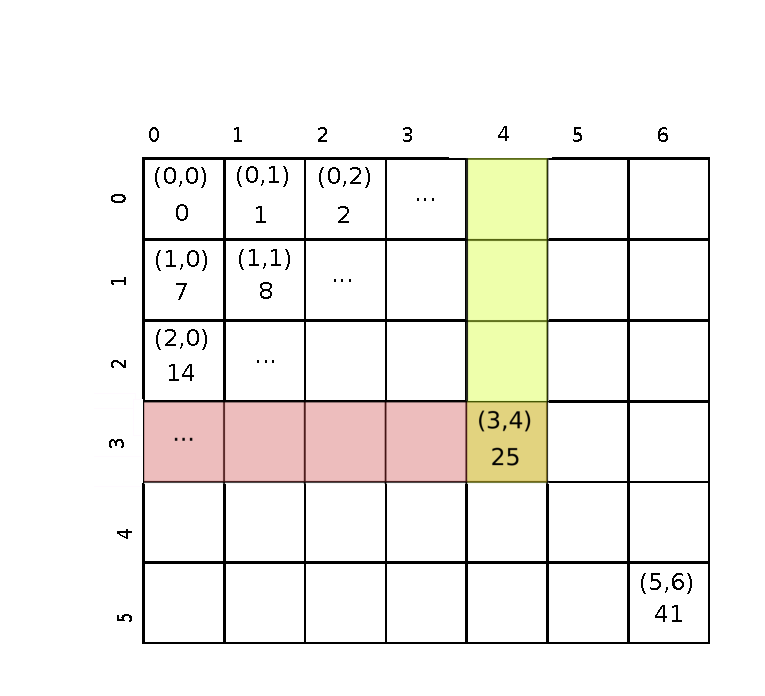
\includegraphics[trim=1.2cm 0cm 0cm 0cm, clip=true]{./images/RowMajor2D}
\caption{Row-major matrix translation}
\label{fig:rowMajor2DExample}
\end{center}
\end{figure}

In figure \ref{fig:rowMajor2DExample} the highlighted cell (3,4) has an offset:
\[
o=d_1*(D_2)+d_2 = 3 \cdot 7 + 4 = 25
\]


\section{Na\"{i}ve implementation}\label{sect:naiveImplementation}
The first attempt of parallelization was performed is a na\"{i}ve porting that yet
incorporates strategies as thread cell mapping that will be the basis of the
more and sophisticated successive versions of the parallelization.
\subsection{Blocks organization}
The whole cellular space was equally divided in \texttt{BLOCK\_SIZE\_X} chunks
of threads on the \textit{x}-dimension and in \texttt{BLOCK\_SIZE\_Y} on the
\textit{y} one. Then each thread within the blocks was mapped to one cell
of the cellular space. We simple used the block and thread indexing provided by
the CUDA framework (see section \ref{kernels}) to implement that kind of
mapping.
More in detail the problem here is to calculate the global index \(o\) (unique)
of the thread given a grid-block organization. As stated before the
launch configuration can be set up with all the combinations of possible
dimensions values for grids and blocks (1 to 3 dimensions each). In particular
here the thread organization used is always:
\begin{itemize}
  \item 2D \textbf{grid} and 2D \textbf{blocks} reflecting the 2D nature of the
  model.
\end{itemize}
so the approach used was to find first a unique couple of indexes mapping to the
2D coordinate of the cellular automata, and then use the formula (see section
\ref{1Dto2Dmemory}) to transform it into the 1D index, needed to refer to 1D
CUDA buffers.

\[col=threadIdx.x+blockIdx.x \times blockDim.x;\]
\[row=threadIdx.y+blockIdx.y \times blockDim.y;\]
\[linearIndex=row \times DIMROW + COL\]



The two values, \texttt{BLOCK\_SIZE\_X} and
\texttt{BLOCK\_SIZE\_Y} are considered in effect parameters and a tuning
phase was needed in order to find the better configuration in terms of
minimizing the execution time.
Obviously is possible to allocate only an integer number of blocks and hence a
simple blocks number calculation like
\[
BLOCK\_NUM\_X=\frac{SIZE\_CELL\_SPACE\_X}{BLOCK\_SIZE\_X} \]
\[
BLOCK\_NUM\_Y=\frac{SIZE\_CELL\_SPACE\_Y}{BLOCK\_SIZE\_Y}
\]
would fail in most of cases (it would work only when\\
\(SIZE\_CELL\_SPACE\_\{X\_Y\}\) is multiple of \(BLOCK\_SIZE\_\{X\_Y\}\)). So
the approach used was :
\[
BLOCK\_NUM\_X=\Bigl\lfloor\frac{SIZE\_CELL\_SPACE\_X}{BLOCK\_SIZE\_X}\Bigl\rfloor + 1 \cdot \alpha\]
\[
BLOCK\_NUM\_Y=\Bigl\lfloor\frac{SIZE\_CELL\_SPACE\_Y}{BLOCK\_SIZE\_Y}\Bigl\rfloor
+ 1
\cdot
\beta
\]

where
\[
\alpha =
\begin{cases}
1 &\mbox{if } \frac{SIZE\_CELL\_SPACE\_X}{BLOCK\_SIZE\_X} \not\in \mathbb{N}  \\
0 & \mbox{otherwise }
\end{cases}
\]
\[
\beta =
\begin{cases}
1 &\mbox{if } \frac{SIZE\_CELL\_SPACE\_Y}{BLOCK\_SIZE\_Y} \not\in \mathbb{N}  \\
0 & \mbox{otherwise }
\end{cases}
\]
For example let \(SIZE\_CELL\_SPACE\_X=500\), \(SIZE\_CELL\_SPACE\_Y=800 \) and
\(BLOCK\_SIZE\_X=16,BLOCK\_SIZE\_Y=8\) be respectively the X and Y dimension
sizes of the cellular space and the X and Y block sizes; the number of blocks is
so calculated:
\[
BLOCK\_NUM\_X=\Bigl\lfloor\frac{500}{16} \Bigl\rfloor + 1 \cdot 1 =
\floor{31.25}+1\cdot1= 31 + 1= 32\]
\[
BLOCK\_NUM\_Y=\Bigl\lfloor\frac{800}{8} \Bigl\rfloor + 1 \cdot 0
=\floor{100}+0= 100 + 1\cdot0= 100 \]
This means that it is possible to ceate more threads
 than the total number of cells that make up the whole cellular space.
Regarding the latter example:
\[
(32\cdot 16) \cdot (100\cdot 8)=409600 > 800 \cdot 500= 400000
\]
meaning that \(409600-400000=9600\) allocated threads are ``superfluous'' in a
context of \textit{one-cell one-thread} mapping and have to be managed into code and taken
into account when designing the porting and evaluating performances.
We handled the bad consequence of this scenario just denying them from
computation within each kernel (see listing \ref{code:wastedThreads})


\lstset{label={code:wastedThreads},caption={Superfluous threads check},
style=codeStyleC }
\begin{lstlisting}
	//calculating 2D coordinate of the cellular
	//space cell to be handled by this specific thread
	int col=(threadIdx.x+blockIdx.x*blockDim.x);
	int row=(threadIdx.y+blockIdx.y*blockDim.y);
	if(col>=0 && col <= SIZE_X){
		if(row>=0 && row <= SIZE_Y){
			/*
			Do work only here
			*/
		}
	}

\end{lstlisting}


\subsection{Race Condition avoiding}\label{sect:raceCondAvoiding}
Some parts of the code are not race condition free, and were re-designed in
order to avoid them. The flows distribution phase, in the serial model, is
designed such that each cell is responsible for updating substates of the
neighbors (see section \ref{sect:sciaraModelTau2}). In a parallel context this
kind of approach is unfeasible due to obvious consequences of modifying the same
memory locations at the same time from within different threads (uncongruences,
dirty reads, etc). Thus, a new substate was added named \textit{flows}
substate that keeps trace of all the flows destinated to the cell. For each cell
and for each substate that need an update 9 variables are reserved, and updated
only once by only one thread and then ``reduced'' by the central cell in order
to compute the final value.

Formally, let \(c\) be the index of the central cell and \(k\) the number of
substates to be threated as race-condition free. Then, for each cell, a buffer of length \(k
\cdot 9 \) is allocated, and each space of it is reserved to store the \(i\)th cell's
contribution to one of the \(k\) state substates. The organization of this
buffer is such that elements from \(ki\) to \(ki +9\) represents
the \(9\) contributions (one from each neighbors) to the \(c\)'s \(i\)th
substate.
It is up to the central cell to reduce all the values within this buffer,
compute the final result and update the correspondent substate after that it
was filled in completely.
In this way no concurrent updates may take place.

\begin{algorithm}
\caption{Substates update}
\begin{algorithmic}
\label{alg:substateUpdate}
\REQUIRE \(f(c,v)\) flow from cell c to neighbor v
\REQUIRE \(vic(c,v)\) \(v-th\) neighbor of the cell \(c\)
\ENSURE \hfill \\
\(k=4 \Leftarrow v=1\) \\
\(k=3 \Leftarrow v=2\) \\
\(k=2 \Leftarrow v=3\) \\
\(k=1 \Leftarrow v=4\) \\
\(k=7 \Leftarrow v=5\) \\
\(k=8 \Leftarrow v=6\) \\
\(k=5 \Leftarrow v=7\) \\
\(k=6 \Leftarrow v=8\) \\
\(k=0 \Leftarrow v=0\) \\
\FORALL{\(c \in CELLSPACE\)}
\FORALL{\(v \in \{0\ldots8\}\)}
\STATE \(SUBST(C) = SUBST(C) - f(c,v);\)
\STATE \(SUBST(C) = SUBST(C) + f(vic(c,v),k);\)


\ENDFOR
\ENDFOR
\end{algorithmic}
\end{algorithm}

All the quantities that flow out to the neighbors have to be subtracted from
the central cell (according to the law of conservation of mass, see
figure \ref{fig:exitingFlows}). Next, all the flows related to that cell have
to be collected and processed. Note that each cell receives only one flow (per
substate) from one neighbor. The cell \(c\) has to collect all the flows that
flow out from the neighbors and are addressed to it. From the point of view of
\(vic(c,1)\), \(c\) is the \(4-th\) neighbor, and that's why \(c\) will collect
\(f(vic(c,1),4)\); the same idea holds for the whole neighborhood (see figure
\ref{fig:exitingFlows} , algorithm \ref{alg:substateUpdate}).



\begin{figure}
\begin{center}
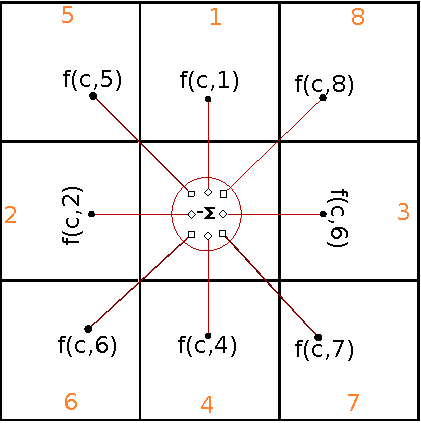
\includegraphics[scale=1.2]{./images/exitingFlows}  \caption{Exiting flows
subtraction from the central cell. In orange the relative index of the
neighbor to the central cell. F(c,v) represent the flow designed for the
neighbor v.}
\label{fig:exitingFlows}
\end{center}
\end{figure}

At the end of this phase all the flow exchanges are already performed and the
model can proceed applying the further elementary functions.

\section{Device occupancy considerations}\label{sect:idleThreadsDevOccupancy}
Device occupancy is a crucial aspect of GPGPU CUDA when addressing the designing
of efficient GPU applications.
It is not possible to achieve high speedup if all the computation resources of
the devices are not fully exploited and on the other hand it is easy to see that
an over utilization leads to inefficient execution as well. The
\textit{na\"{i}ve implementation} we have seen in section
\ref{sect:naiveImplementation}, that always allocates as many threads as the
dimension of the whole cellular space, most of the time over utilizes the device
when there's no need to, hence executing the model in a not optimal way.
When considering a phenomenon (i.e., a lava flow) that is topologically
connected (i.e., a simulation starts from few active cells and evolves by
activating neighbour cells), the CA execution can be drastically accelerated
restricting the application of the transition function to the only
\textit{active} cells\footnote{Optimization that is related also with the
SCIARA-fv3 CA sequential version \cite{Walter2004}}.

In general the area interested by a lava flow is a growing portion (smaller) of
the whole space, so there's no need to allocate as more threads as the number of
cells of the area, because no flow cannot be generated without lava presence.
Allocated threads are resource demanding and consuming, and when the total
number exceeds the number of processors they have to be scheduled serially, with
the obvious consequences in terms of performance slowdown.
For example, in the run of the model on a dataset coding Mt Etna's 2006
eruption\footnote{On 14 July 2006 at 2330 hr a fissure opened on the east flank
of the Southeast Crater. Two vents along the fissure produced a lava flow which
spread 3 km east to the Valle del Bove. The eruption ended on 24 July.} (see
figure \ref{fig:etnaEruption1} ) the lava maximum expansion does not interest
more than the \(8\%\) of total cells are interested, meaning that the \(92\%\)
of threads are IDLE (those values hold even if the real event map is compared
with the portion of the dataset taken in account by the cellular space).
\begin{figure}
\begin{center}
  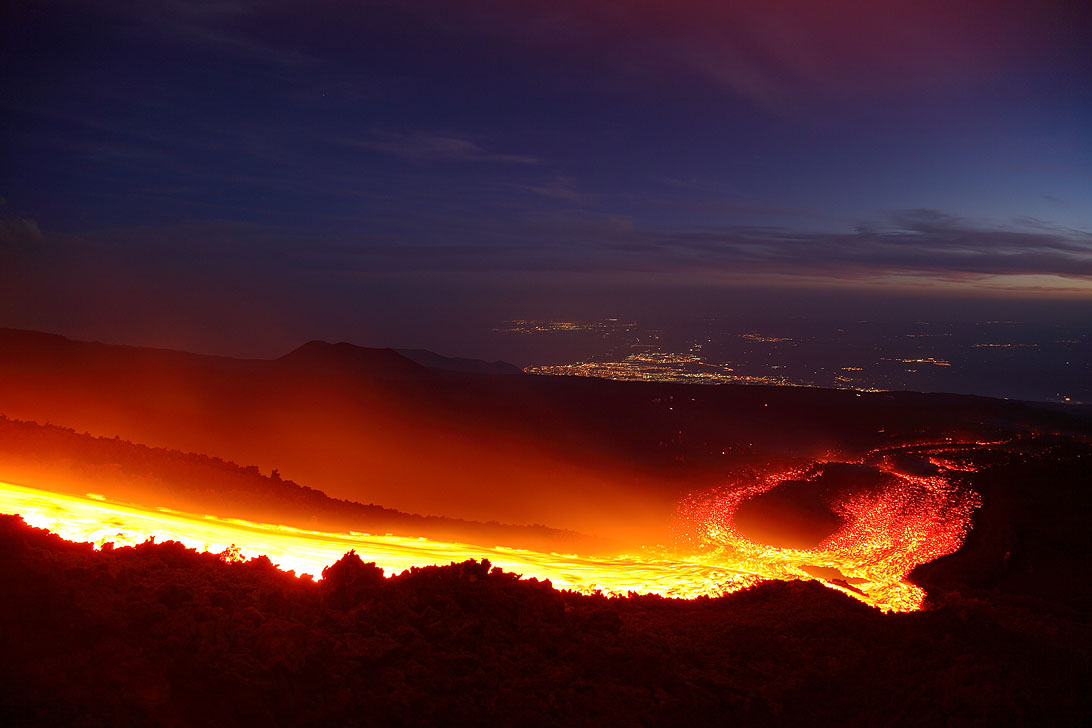
\includegraphics[scale=1.50]{./images/etna2006PictureEruption1}
  \caption{Etna 2006 eruption.}
  \label{fig:etnaEruption1}
\end{center}
\end{figure}

An approach that dynamically adapts the grid of threads with the current lava
distribution among cells may solve this issue, hence a serial (if any) thread
execution is consequence of a real computation. Section
\ref{sect:RBBOptimization} and \ref{sect:linearCellAtomic}  present two
 different approaches that try to mitigate the problem of IDLE cells.

\section{Rectangular Bounding Box - RBB}\label{sect:RBBOptimization}
The first adopted strategy utilize a Rectangular Bounding Box (RBB) within which
all the active cells reside. As the lava flows and invades more space it
dynamically grows, hence is not necessary to launch as many threads as the
number of cell in the whole cellular space, but it is sufficient to allocate
only those ones that compute the transition function for the cells within the
RBB.
This drastically reduces execution times, since the sub-rectangle is usually
smaller than the original CA space, leading to a more efficient utilization of
the device resources.


For this reason, a GPU optimized CA (GPU-OCA) version has
been tested that takes into account, at each CA step, the RBB
that includes all active cells (i.e., cells containing lava) of the
automaton. However, while in a sequential OCA (CPU-OCA)
the CA space matrix is simply scanned by considering the
RBB boundaries instead of the whole CA, the GPU-OCA must
consider the rectangular grid bounding box (RGBB) containing
active cells, which in general includes the traditional RBB of
active cells (see figure \ref{fig:RBB}).

\begin{figure}
\centering
  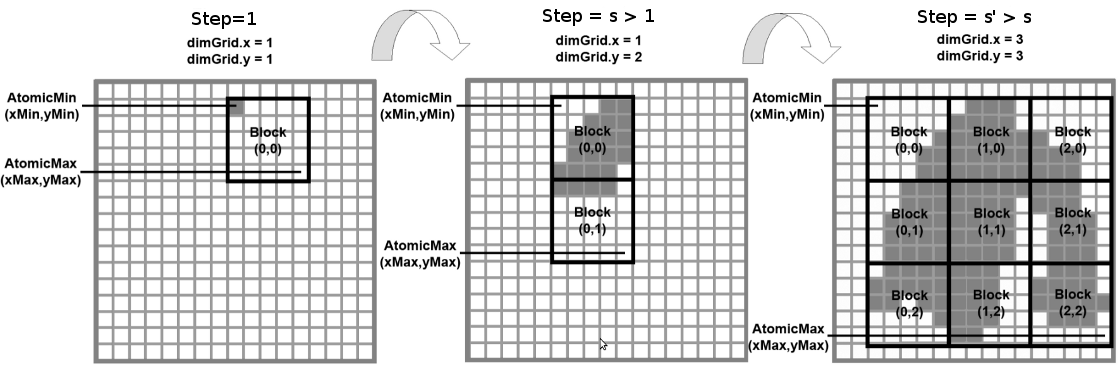
\includegraphics[scale=0.4]{./images/RBB}
  \caption{An example of dynamic RGBB (rectangular grid bounding box) expansion, referred to a 5 x 5 block size grid. As lava expands, blocks interested by
active cells are activated.}
  \label{fig:RBB}
\end{figure}

However, while in a sequential OCA (CPU-OCA) the CA space matrix is simply
scanned by considering the RBB boundaries instead of the whole CA, the GPU-OCA
must consider the rectangular grid bounding box (RGBB) containing active cells,
which in general includes the traditional RBB of active cells (Figure
\ref{fig:RBB}) that has been implemented storing a double copy of an array of 4
indexes that keep trace of the size of the rectangle, one for reading and the
other for updating.
During the distribution phase (the only time the RBB may increase its sizes),
when a newly activated cell resides out of the RBB's bounds, an atomic CUDA
operation (\texttt{atomicExch(\ldots)}) is performed in order to update the RBB.
At the end of the distribution phase the two arrays are swapped, so the subsequent
elementary processes will work also on the new active cells.

The grid of blocks grows dynamically as the simulation is carried on, so at each
CA step, the grid of threads readapts itself by creating a new block of threads as
soon as the RBB is interested by a newly activated cell (see figure
\ref{fig:RBB}) out of its boundaries.
Thus, since the overall number of launched kernels is reduced,
the computational performance of the algorithm improves significantly.


\lstset{label={code:memoryPattern2D}, caption={Rectangular bounding box
management phase. Each new activated cell checks whether its indexes are out of
the RBB, and if it is true,  they update the box boundaries.}, style=codeStyleC
}
\begin{lstlisting}
	/*distribution phase terminate here*/
	if(d_nSh[index] > 0 ){	
		if (col <= D_SCAL->minRect[0]-1)
			atomicExch(&D_SCAL->minRect[5],col);
		if (col >= D_SCAL->minRect[1]+1)
			atomicExch(&D_SCAL->minRect[6],col);
		if (row <= D_SCAL->minRect[2]-1)
			atomicExch(&D_SCAL->minRect[7],row);
		if (row >= D_SCAL->minRect[3]+1)
			atomicExch(&D_SCAL->minRect[8],row);
	}
\end{lstlisting}

Notwithstanding this operation is implemented by means of atomic CUDA
instructions, it does not represent a bottleneck (atomic operations in CUDA have
to be used with caution, see section \cite{NvidiaprogGuide}) because each RBB
update is performed only once (per RBB's side) and, considering that the RBB
increases its sizes of maximum one unit per dimensions at each CA step, it is
easy to see that the first cell that updates a border (e.g.
\texttt{D\_SCAL->minRect[5]}, the top border, for example) disables all the
others threads to execute further modifications on that variable.


Despite the good performance improvements that were achieved, figure
\ref{fig:RBBSchreenShot} shows, that in some cases, the RBB approach is not
optimal\footnote{This is not the case when the lava spreads
homogeneously in a square pattern, which usually does not hold for real
events.} in limiting the number of IDLE cells.
Even within the boundaries of the rectangle the percentage of active cells is
still low due the box expansion policy. The boundaries can be expanded due to
the activation of a few number of cells (one is sufficient) on the RBB frame,
but the entire row and column in which they reside will be scheduled
for execution.
For example, regarding figure \ref{fig:RBBSchreenShot}, if a cell on the bottom
right corner was activated, it would produce a RBB size increase consisting of a
whole column and row despite the activation of only one cell.



\begin{figure}
\begin{center}
  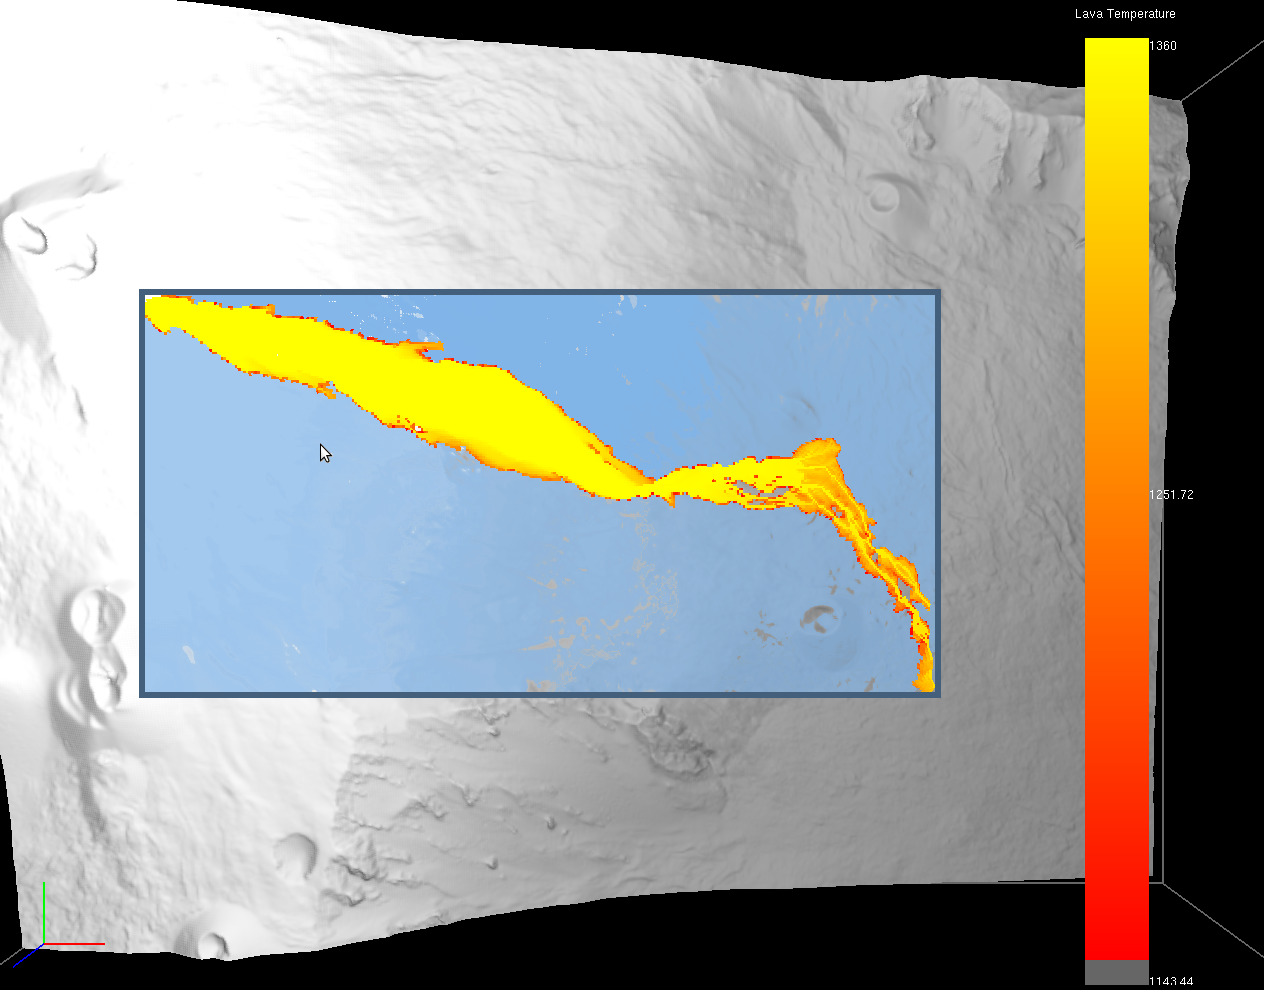
\includegraphics[scale=0.35]{./images/RBBSchreenShot}
  \caption{A screenshot from the SCIARA-fv3 model lava flow visualizer showing
  the RBB in action. Only the portion of the cells within the RBB are
  actually }
  \label{fig:RBBSchreenShot}
\end{center}
\end{figure}

\section{Atomic Functions implementation}\label{sect:atomicImplementation}
Atomic operations\cite{NvidiaprogGuide} (see section \ref{chap:CUDA}) are
essential in multithreaded programming, especially when different threads need
to read or write the same data location. Conventional multicore CPUs generally
use a test-and-set instruction to manage which thread controls which data. CUDA
has a much more extensive set of atomic operations\footnote{Even the C/C++
construct \texttt{foo++} looks like a single operation, but in reality, the
hardware might carry out three separate steps when performing the increment:
 \begin{inparaenum}
\item fetch foo into a register, 
\item increment the register by one, and
\item write the register back to foo in global memory. Without a lock, two or more parallel threads might
simultaneously read foo into a register at the same time, which means they would
be unaware of the increment in progress by the other threads
\end{inparaenum}} but, in a parallel environment they represent a real
challenge because they serialize the execution flow.
In other words, incrementing a single counter with \texttt{atomicAdd()} means
that the counter has to be locked, thus forcing all threads to stop and wait in
order to individually perform the increment operation — one after the other; it
is the antithesis of parallel programming. The goal, when using this kind of
operation is to design \textbf{low-wait} algorithms, s.t. the number of threads
that must wait for the lock to be released is kept to the minimum and, at the
same time, maximixing the active threads number.\footnote{NVIDIA SDK
histogram example\cite{NvidiaprogGuide}, at \url{http://docs.nvidia.com/cuda/cuda-samples/#cuda-histogram}, demonstrated a
form of low-wait algorithm via the use of a vector of counters that are
incremented with \texttt{atomicAdd()} operations.}


With CUDA, one can effectively perform a test-and-set using the
\texttt{atomicInc()} instruction or use atomic operations as well, to actually
manipulate the data itself, without the need for a lock variable.
 
Atomic functions have to be used with caution also due to another possible
 performance side-effect:
when operating from global memory they are not cached.
This means that every time an atomic operation is performed there must be a
read from the global memory, and if the value needs to be modified, there must
be a write to global memory too. This can take hundreds of clock cycles to
accomplish.
The CUDA architecture is set up to withstand extreme latency but, if too
many threads are stalled, the computational throughput of the GPU will severely
diminish.

Atomic functions were successfully employed in solving the problem of race
conditions faced in section \ref{sect:raceCondAvoiding}. They open the
possibility of utilize the original (see section
\ref{sect:sciaraModelTau2}) lava distribution schema across the cells instead the creation and management of another substate. They allow a more
direct and easy porting, because the responsibility of the computational
coherence rely on the CUDA framework instead on the programmer.
The implementation is such that during the distribution phase each substate is
managed via atomic functions. An example in listing
\ref{code:atomicDistribution} shows how a cell distribute quantities to its
1-th neighbor (the same concept holds for the whole neighborhood).

\lstset{label={code:atomicDistribution}, caption={Distribution phase across
cells related to the 1th neighbor of the index-th central cell.   },
style=codeStyleCUDA }
\begin{lstlisting}
	int lungCOL=d_params[EN_LY];
	float cache=d_outFlwPriv[getPrivateVarIdx(index,0,1)];
	int idxNeigh=getNeigh1(index,lungCOL);
	if (cache > 0){
		//central cell lava flow subtraction 
		atomicAdd(&d_nSh[index],-cache);
		//neighbor - lava flow
		atomicAdd(&d_nSh[idxNeigh],+cache);
		//neighbor - momentum along x-axis
		atomicAdd(&d_nSpx[idxNeigh],cache*d_outFlwPriv[getPrivateVarIdx(index,1,1)]*COS_ALPHA_1);
		//neighbor - momentum along y-axis
		atomicAdd(&d_nSpy[idxNeigh],cache*d_outFlwPriv[getPrivateVarIdx(index,1,1)]*SIN_ALPHA_1);
		//central cell temperature subtraction 
		atomicAdd(&d_nST[index],-cache*d_ST[index]);
		//neighbor - temperature
		atomicAdd(&d_nST[idxNeigh],cache*d_ST[index]);
 		...
}
\end{lstlisting}

Despite its simplicity, this approach does not allow the utilization (on the
available hardware) of double precision buffers, because the framework does not
expose any \textit{official}\footnote{An alternative solution for double
precision atomic addition exists and were tested as well despite the well-known
related performance issue. Code in listing \ref{code:doubleAtomic} at page
\pageref{code:doubleAtomic}.} support  for atomic operations on double.
It will be shown in section \ref{sect:precisionConsid} that in SCIARA-fv3,
double precision may be crucial for the correctness of final result.
A different discussion is reserved for atomic operations on \textit{Kepler}
family GPUs that are more efficient than on \textit{Fermi} GPUs insomuch 
they can often be processed at rates similar to global load
operations\footnote{Throughput of global memory atomic operations on Kepler is
substantially improved compared to the Fermi generation by 9x to one operation
per clock throughput to independent global addresses is also significantly
accelerated, and logic to handle address conflicts has been made more efficient
as well.
This speed increase makes atomics fast enough to use frequently within kernel
inner loops, eliminating the separate reduction passes that were previously
required by some algorithms to consolidate results. Kepler GPUs also expands the
native support for 64-bit (double precision) atomic operations in global
memory.}.


Note that within this setting each substate value of each cell may be modified
by a maximum number of 9 threads per step (the whole neighborhood itself) meaning
that the global memory substate updates of a cell may stall not more
that 9 threads, so it is possible to classify this approach as low-wait.
In addition, in real case simulation it is very improbable that at each step
all the active cells are interested by all the 9 outflowing flows, and this
furtherly decreases the overall serialization rate.




\section{List of active cells implementation}\label{sect:linearCellAtomic}
This section describes a totally different approach that tries to solve the
problem of IDLE cells. As seen in section \ref{sect:RBBOptimization} RBB may
be a valid solution, but could not be efficient in several situations. The
\textit{list of active cells - LAC} approach is built on top of the atomic
implementation described in section \ref{sect:atomicImplementation}. It is
based on the concept that only the active cells have to be processed by CUDA
threads.

In this version a list of cell indexes is managed by the program, and whenever a
new cell is activated by means of some lava quantity it is added to that list in
order to be processed by one of the allocated thread.
In this way it is possible to keep track of the size of the LAC and launch only
the necessary number of threads onto the device.  If at the time \(t\) there are
\(NC\) active cells, the corresponding LAC list will have size \(NC\). The
\(i^{th}\) allocated thread will handle the cell of index \(LAC(i)\) at position
\(i\) of the list. Thread index and CA cell index are in this case completely
disassociated, disabling the possibility of using the distribution method
utilized so far and described in the algorithm \ref{alg:distribution} at page
\pageref{alg:distribution}.
 In theory no waste of computational resources may take place, but other factors
 have to be considered, first and foremost global memory coalescence (see
 section \ref{memoryModel}) because cells are not activated in a prefixed order
 (in terms of same computational step or of cells that trigger their
 activation), and hence their order in the LAC list could not reflect the real
 topological proximity, meaning lots of unnecessary global memory
 accesses.
 Coalescence may be ``improved'' simply ordering the LAC
 regularly\footnote{Finding the right tradeoff between the cost of ordering and
 resulting coalescence benefits is a key concept here.} within the execution.
 
 %Figure \ref{fig:LACExample} shows an example of the LAC order-proximity
 %relation and related coalescence problems.
 For example, let's suppose that \(C\) is a \(n \times m = 3\times 3\)
 bi-dimensional cellular space and that at time \(t\) only cell \(i\) is active and at time \(t+1\) it
 triggers the activation of cells (in order) \(\{i-3,i+2,i+4\}\) and at time
 \(t+2\) of the cells \(\{i+1,i-2,i+3,i-4\}\).
 The LAC list would be : \(LAC=\{i,i-3,i+2,i+4,i+1,i-2,i+3,i-4\}\)

\begin{center}
\begin{tikzpicture}
\draw[step=2cm,color=black] (0,0) grid (6,6);
\matrix[matrix of nodes,
inner sep=0pt,
anchor=south west,
nodes={inner sep=0pt,text width=2cm,align=center,minimum height=2cm}
]{
\(i-4\) & \(i-3\) & \(i-2\) \\
\(i-1\) & \(i\) &  \(i+1\) \\
\(i+2\) & \(i+3\) & \(i+4\)  \\
};
\end{tikzpicture}
 \end{center}
hence \(n \times m = 3\times 3 = 9\) threads will be created and launched with
indices \(T=\{0,1,2,3,\ldots,8\}\). They execute the transition
function on cells of LAC in such manner that \(T(i)\) manages cell
\(LAC(i)\)\footnote{In reference to the previous example: 
\((T(0),LAC(0)=i),(T(1),LAC(1)=i-3),(T(2),LAC(2)=i+2)\ldots\)}.
Obviously, two ``contiguous'' threads execute on two discontiguous memory
locations, disabling coalescence. What was devised, in order to
mitigate this issue and keep getting advantage of the low number IDLE threads, is to sort
the \(LAC\) thus realizing the topological proximity whithin the buffer 
and making both threads and cells well ``coupled''.
The activation is obtained adding the index of the cell to the LAC (see
listing \ref{code:LACactivation}).
\lstset{label={code:LACactivation}, caption={Cell activation in LAC approach. 
}, style=codeStyleCUDA }
\begin{lstlisting}
	__device__ void ActiveCell(int col, int row, SCALARS_GPU* D_SCAL,int * d_ACT,int*d_indexCelleAttive){
		int index=linearizedIndex(col,row,d_params[EN_LY]);
		int old;
		if (!d_ACT[index]){
			old=atomicExch(&d_ACT[index],1);
			if(old==0){
				atomicExch(&d_indexCelleAttive[atomicInc((unsigned int*)&D_SCAL->minRect[9],NUMCELLS)],index);
				
} } }
\end{lstlisting}
Moreover other overheads may be introcuced by the fact that an atomic operation
is required since two or more threads may activate a cell at the same time and
hence write the same LAC location.




\section{Shared memory optimizations}\label{sect:sharedMemoryOptimization}
Shared memory (SM) was exploited in order to take advantage of its higher
speed \footnote{As known, access to a location in 
shared memory of each multiprocessor has 
a much lower latency than that carried out 
on the global device memory, see section \ref{shareMemory}}.
For this 
reason, an accurate analysis was carried out in 
determining how much memory accesses each 
thread performs for each CA substate matrix, 
in order to evaluate the convenience of using SM. This 
investigation gave rise to a ``hybrid'' memory access pattern, where shared memory 
allocation was adopted in those kernels accessing CA substate matrixes at least
three times\footnote{Considering that using shared memory implies its
management, and thus two global memory accesses (initialization from, and write
back to global memory).}

On this basis, the data buffers corresponding to the elevation, lava thickness
and temperature and distributed outflows (\(Q_h \;, Q_T \;, 
Q_o\;, outflows \)) were allocated in SM.

Let's briefly show an example of SM usage, its initialization,
utilization and finalization.
SM has to be initilizated each time a kernel executes (see listing
\ref{code:sharedMemoryInitialization} as example code).

\lstset{label={code:sharedMemoryInitialization}, caption={Shared memory
initialization from Global Memory. }, style=codeStyleCUDA }
\begin{lstlisting}
	__shared__ double s_Sz[(blockDimY+2)][(blockdimX+2)];
	__shared__ double s_Sh[(blockDimY+2)][(blockdimX+2)];
	... 
	if(threadIdx.x==0){
		s_Sz[threadIdx.y+1][0]=d_Sz[getNeigh2(index,lungCOL)];
		s_Sh[threadIdx.y+1][0]=d_Sh[getNeigh2(index,lungCOL)];
	}

	if(threadIdx.x==blockDim.x-1){
		s_Sz[threadIdx.y+1][blockDim.x+1]=d_Sz[getNeigh3(index,lungCOL)];
		s_Sh[threadIdx.y+1][blockDim.x+1]=d_Sh[getNeigh3(index,lungCOL)];
	}
	//cell inside borders of the block(plus ghost cells)
	s_Sz[threadIdx.y+1][threadIdx.x+1]=d_Sz[index];
	s_Sh[threadIdx.y+1][threadIdx.x+1]=d_Sh[index];

	__syncthreads(); //shared has to be fully initializated before computation takes
	//place. end shared loading
\end{lstlisting}

After it has been initializated it can be used normally in place of GM, but at
the end of the computation (SM is cancelled each time a kernel ends), if one
wants to keep some value in memory, a copy from SM to GM has to be performed.



\section{If divergences mitigation}
Here is briefly shown a tecnique that may be useful for the mitigation of
thread divergenge due to \texttt{if} statements.
This simply consists in letting all threads execute all instructions within all
\texttt{if} statements, ensuring that the final value of the variables is the
same as if would have been computed inside the \texttt{if}s.
See as example, how listing  \ref{list:ifDivergence1} is converted in an
equivalent \texttt{if}-free code (listing \ref{list:ifDivergence2}) as example :

\lstset{label={list:ifDivergence1},caption={If divergent example code},
style=codeStyleC }
\begin{lstlisting}
		if (d_Spy[index] >= 0){
			alpha_p = acos(d_Spx[index]/d_outFlwPriv[getPrivateVarIdx(index,12,0)]);
		}else{
			alpha_p = 2.0*PI_GRECO - acos(d_Spx[index]/d_outFlwPriv[getPrivateVarIdx(index,12,0)]);
		}
\end{lstlisting} 



\lstset{label={list:ifDivergence2},caption={Converted if-free section},
style=codeStyleC }
\begin{lstlisting}
	condition=d_Spy[index] >= 0;
	alpha_p= -(condition*-(2.0*PI_GRECO)+ acos(d_Spx[index]/d_outFlwPriv[getPrivateVarIdx(index,12,0)]));
\end{lstlisting} 
It's easy to see that whether \(d\_Spy[index] >= 0\) is greater equal than
\(0\) the final value of the variable \(alpha\_p\) is equivalent between the two
listings (a boolean value \tcondition is internally represented in C as
\(0=false\) and \( a=true,\; a>0\)).
It is known that GPUs devote  more transistors than CPUs  to computation
instead of control flow, so in some situations a gain in performance using this
tecnique may take place. Experimentations, anyway, have to be performed in order
to find the best set of \texttt{if}s to be converted and evaluate real
performance gain obtained.
Note that in general converted code, expecially ones with several nested
\texttt{if}s, becomes less readable and maintenable.




\section{Test, validation and performances results}

  Two devices were adopted for testing
different versions of CUDA implementations of the Sciara-fv3 model, the GTX 580 (Fermi architecture) and GTX 680 (Kepler
architecture) graphic processors (see section \ref{sect:keplerArch} at page
\pageref{sect:keplerArch}). In particular, the latter has 1536 CUDA cores, 2 GB
global memory and 192 GB/s high-bandwidth communication between CPU and GPU,
while the former device has 512 cores 192 GB/s high-bandwidth. The sequential
SCIARA reference version was implemented on a 3.4 GHz Intel Core i7 based
desktop computer. As previously stated, the sequential reference CPU version is
fully-optimized, where each cell can update neighbour cells directly.
At the contrary, parallel versions introduce flow substates with the inevitable
addition of overheads. However, an optimization regards both versions: at every
step, the CA space array is scrolled and the transition function applied to each
cell of the CA only where lava is present, skipping \textsl{empty} cells.
A first test regarded the simulation of well-known and documented real lava flow
event, the Mt. Etna 2006 lava event occurred in July 14, 2006, where the CA
space is a $517 \times 378$ two-dimensional grid. Besides, two different memory
layouts were considered, by adopting a hybrid shared-global memory as explained
in the previous section and all-global version.
Simulations were carried out for 370.000\footnote{At this step the simulation is
almost completed, it means that all the emitted lava has been solidified.} steps
and considering two craters for lava flow emission.
In order to further stress the efficiency of the GPU version, a further
benchmark experiment was performed by considering a $400^2$ cells flat plane
with a central crater. Eventually, some experiments were carried out by adopting
CUDA's intrinsic function (i.e., \texttt{fast\_math} compiler option) feature
(\cite{NvidiaprogGuide}) for single-precision calculations, that permits the use
of mathematical functions that CUDA directly maps on-chip and thus are faster
versions of the corresponding standard ones, even if less
accurate\footnote{Only available for single-precision variable and operations.}.
Timings reported for the considered GPU devices (see Tab.
\ref{tab:execAHM_LAC} and Tab. \ref{tab:execGM_HM} for the GTX 580 and
GTX 680 and GTX 480) indicate their full suitability for parallelizing CA
models. Even if applied to a complex CA model and considering a fully optimized
reference sequential version, performance results show the good computational
power of the considered GPU in terms of execution time reduction, significantly
(and always) outperforming the CPU (sequential) implementation up to $31\times$
for the considered datasets.


{\footnotesize
\begin{table}
\caption{Achieved speedup values of experiments carried out for evaluating the
performance the GPU version of the SCIARA-fv3 MCA lava-flow model on the GTX 580 (Fermi architecture) and the GTX 680 (Kepler architecture) graphic hardware, using the hybrid  memory (HM) and global (GM) memory layouts, fast\_math option (HM\_FM) and by considering single and double precision variable values. A Intel i7-2600 based hardware was adopted for reference sequential tests. The $517 \times 378$ matrix refers to the 2006 Mt. Etna event.} \center
\label{tab:execGM_HM}
\begin{center}

\begin{tabular}{ccccc}
& & \textit{GTX 480 - Hybrid Memory} & &\\
\hline
CA dim &   HM (float) & HM\_FM (float) & HM (double)\\
\hline
$517 \times 378 $ & 14.29 & 14.2 &  9.0  \\
$400 \times 400 $ & 27.12 & 28.1 & 19.4  \\
\hline
\end{tabular}

\vspace{10pt}

\begin{tabular}{ccccc}
& & \textit{GTX 480 - Global Memory} & &\\
\hline
CA dim &   GM (float) & GM\_FM (float) & GM (double)\\
\hline
$517 \times 378$ & 12.55 & 12.56  & 8.13 \\
$400 \times 400 $ & 23.83 & 24.56 & 17.41 \\
\hline
\end{tabular}

\vspace{20pt}
\begin{tabular}{ccccc}
& & \textit{GTX 580 - Hybrid Memory} & &\\
\hline
CA dim &   HM (float) & HM\_FM (float) & HM (double)\\
\hline
$517 \times 378 $ & 15.6 & 15.8 &  10  \\
$400 \times 400 $ & 29 & 31 & 21  \\
\hline
\end{tabular}

\vspace{10pt}

\begin{tabular}{ccccc}
& & \textit{GTX 580 - Global Memory} & &\\
\hline
CA dim &   GM (float) & GM\_FM (float) & GM (double)\\
\hline
$517 \times 378$ & 13.8 & 13.6  & 9.3 \\
$400 \times 400 $ & 28 & 29 & 20.4 \\
\hline
\end{tabular}

\vspace{20pt}

\begin{tabular}{ccccc}
& & \textit{GTX 680 - Hybrid Memory} & &\\
\hline
CA dim &   HM (float) & HM\_FM (float) &  HM (double) \\
\hline
$517 \times 378$ & 8.3 & 8.3 & 6.6  \\
$400 \times 400 $ & 19.5 & 19.3 & 14 \\
\hline
\end{tabular}

\vspace{10pt}

\begin{tabular}{ccccc}
& & \textit{GTX 680 - Global Memory} & &\\
\hline
CA dim &   GM (float) &  GM\_FM (float) & GM (double) \\
\hline
$517 \times 378$ & 7.3 & 7.3 & 6.6 \\
$400 \times 400 $ & 18.5 & 17.6 & 12.3 \\

\hline
\end{tabular}


\end{center}
\end{table}
}




\subsection{Kepler vs Fermi performance}
Results referred to hybrid memory implementations (HM speedups in Tab.
\ref{tab:execGM_HM}) show how the use of
shared memory can improve performances up to 15\%, with respect to the
implementation that considers only global memory (GM speedups in Tab.
\ref{tab:execGM_HM} ) for CA space
allocation. In addition, the use of the \texttt{fast\_math} option has not
produced expected benefits in terms of performances, especially for the
high-performing GTX680, probably due to the relative low computational intensity
rate of the model. Unexpectedly, experiments executed on the GTX580 have
outclassed simulations that were performed on the GTX 680: even in this case,
this is probably due to the adopted non optimal CUDA occupancy for the
considered hardware \cite{Kirk2010}. Another reason might be that the
GTX680, though having a number of cores nearly triple respect to the GTX580, has
a lesser CUDA core clock-rate (1006Mhz vs. 1544Mhz of the GTX580). Moreover, as
shown by different benchmarks, the GTX680 has proven to be more suitable for 3D
graphic applications than for numerical computations \cite{gurusite2013}.



\subsection{Float-Double precision considerations}\label{sect:precisionConsid}
Other experiments were performed to test if single-precision data can be
considered sufficient for SCIARA simulations by comparing results produced by the GPU
version with those produced by the CPU (sequential) version with single
precision data (i.e., \verb"float" type variables), and those produced still by
the same GPU version against a double precision CPU implementation (i.e.,
\verb"double" type variables). In each case, comparison results were
satisfactory, especially for the double-precision versions, where the areal
extensions of simulations resulted the same, except for few errors of
approximation in a limited number of cells. As expected, speed-up measurements
were better for float-value implementations, even if more approximation errors
were present with respect to the corresponding double-value version.

{\footnotesize
\begin{table}
\caption{Achieved speedup values of experiments carried out for evaluating the
performance the GPU version of the SCIARA-fv3 MCA lava-flow model on the GTX
480 (Fermi architecture) and the GTX 680 (Kepler architecture) graphic hardware,
using the Atomic function hybrid  memory (AHM) and the LAC hybrid memory (LAC)
A Intel i7-2600 based hardware was adopted for reference sequential tests.
The $517 \times 378$ matrix refers to the 2006 Mt. Etna
event.}\label{tab:execAHM_LAC} \center
\begin{center}

\begin{tabular}{ccc}
&  \textit{GTX 680 - AHM + LAC} & \\
\hline
CA dim &   AHM (float) &  LAC (float)  \\
\hline
$517 \times 378$ & 12.3 & 14.3  \\
$400 \times 400 $ & 21.7 & 20.8  \\

\hline
\end{tabular}

\vspace{10pt}

\begin{tabular}{ccc}
&  \textit{GTX 480 - AHM + LAC} & \\
\hline
CA dim &   AHM (float) &  LAC (float)  \\
\hline
$517 \times 378$ & 19.9 & 21.5  \\
$400 \times 400 $ & 27.3 & 26.5  \\

\hline
\end{tabular}


\end{center}
\end{table}
}


\subsection{Approximation and numerical errors}
Validation of the parallel models has been tricky also due to differences (at
first sight unexpected) in substate values that were not caused by
implementation errors. 
It has been seen that, different runs of the ``\textit{atomic}'' version,
showed errors growing in the course of CA execution.
The source of errors resides in the order of execution of the operations of
sums and multiplications, that is completly out of control of the programmer in
this ``\textit{atomic}''-based version.
In fact, CUDA atomic operations ensure ``thread safe'' accesses to variables,
but the order in wich they take place is unknown. 
It is well known that \(A+(B+C) \neq (A+B)+C\) in the general case holds
(floating-point operations, as defined in the IEEE-754 standard, are not
associative), and that the ordering of large numbers of operations (such as summations) that deal
with operands of substantially different magnitudes can significantly affect the
final result \cite{Villa_effectsof}\footnote{Small amounts of lava that flow
from one cell to another, summed to the one already present, that is
much greater.}.
On massively multi-threaded systems, the
non-deterministic nature of how machine floating point operations are
interleaved, combined with the fact that intermediate values have to be rounded
or truncated to fit in the available precision leads to non-deterministic
numerical error propagation.
This is the case of SCIARA-fv3 where for a cell \(c\) this kind of error
propagates for hundred of thousands steps, making it big enough to be relevant
in computing substate values.
Problems of this kind have comed out in this version of the model because it is
much more numerical sensitive, being more physically accurate in modelling the
flows.
The problem, hence, does not derive from the parallel implementation and to
confirm this hypothesis another order of execution of the distribution phase was
tested on the sequential version (seen in listing \ref{code:skypIdleCell}), simply
swapping the two \texttt{for} statements of the cells general loop and
comparing the result after a certain number of steps with the original version.
Even the sequential implementation show the same numerical problems.

The magnitude of this error was investigated and results showed (using the
dataset of Mt Etna) that after \(350000\) steps the \(\cong80\%\) of the cells
had and error less or equal to the \(10\%\) respect to the sequential version,
meaning a difference of the order of \(10^{-2}\;m\).
However, in the context of complex macroscopic phenomena, and in particular in
context of lava flow simulation, errors of this kind are insignificant.


